\documentclass[a4paper,10pt]{article}
\usepackage[utf8]{inputenc}  %support direct writing of German Umlauts

\usepackage{bm}
\usepackage{amssymb}
\usepackage{amsmath, amsthm}
\usepackage{url}

\usepackage{algorithm2e}

\usepackage{pmboxdraw}
\usepackage{verbatim}
\usepackage{multirow}

\usepackage{textcomp}
\usepackage{siunitx}

\sisetup{
  per-mode=symbol,
  binary-units=true
}
\usepackage{booktabs}

\usepackage[usenames,dvipsnames]{xcolor}
\usepackage[normalem]{ulem}

\usepackage{fullpage}

\usepackage{longtable}

\definecolor{dkgreen}{rgb}{0,0.6,0}
\definecolor{gray}{rgb}{0.5,0.5,0.5}
\definecolor{mauve}{rgb}{0.58,0,0.82}

\usepackage{listings}

\lstset{language=C,
        frame=single,
        keywordstyle=\color{blue},
        commentstyle=\color{dkgreen},
        stringstyle=\color{mauve},
        basicstyle=\footnotesize,
        captionpos=b,
        morekeywords={*,command, event, interface},
        tabsize=4,
        columns=fullflexible
}

\usepackage{rotating}

\usepackage{tikz}
\usetikzlibrary{calc,shapes,arrows,decorations.pathreplacing, intersections}


\usepackage[tikz]{bclogo}

\newcommand{\sdcard}[0]{SD Card\xspace}
\newcommand{\edit}[1]{{\color{Red} #1}}
\newcommand{\deledit}[1]{\sout{#1}}

\newenvironment{todo}[1][TODO]{%
	\begin{bclogo}[noborder=true,logo=\bcpanchant]{#1}
}
{\end{bclogo}}
\newenvironment{note}[1][Note]{%
	\begin{bclogo}[noborder=true,logo=\bcinfo]{#1}
}
{\end{bclogo}}
\newenvironment{hint}[1][Hint]{%
	\begin{bclogo}[noborder=true,logo=\bclampe]{#1}
}
{\end{bclogo}}
\newenvironment{attention}[1][Attention]{%
	\begin{bclogo}[noborder=true,logo=\bcattention]{#1}
}
{\end{bclogo}}

\newcommand{\pts}[2]{\textbf{[#1]} #2}

\renewcommand{\ge}[0]{\geqslant}
\renewcommand{\le}[0]{\leqslant}
\renewcommand{\geq}[0]{\geqslant}
\renewcommand{\leq}[0]{\leqslant}

\usepackage[colorlinks]{hyperref}
\usepackage[capitalize,nameinlink,noabbrev]{cleveref}
\crefname{lstlisting}{Listing}{Listings}

\def\uintF{uint16\_t}
\def\uint8{uint8\_t}
\def\intF{int16\_t}
\def\int8{int8\_t}

\newcommand{\module}[1]{\textbf{#1}}
\def\interface#1{{\em #1\/}}

\newcommand{\TStrut}{\rule{0pt}{2.4ex}}

% \usepackage{draftwatermark}
% \SetWatermarkLightness{0.92}
% \SetWatermarkText{DRAFT}
% \SetWatermarkFontSize{10cm}
% \SetWatermarkScale{5}

%opening
\title{MCVU 2018 -- Application 2\\TinyOS Radio scanner{\small{v1.0}}}

\author{}
\date{}

\begin{document}

\maketitle


\begin{center}

\begin{tabular}{|r|c|l|}
\hline
Version & Date & Remark \\
\hline
\hline
%1.1 & Jun 13, 2017 & Update of scoreboard Interface \\
1.0 & Dec 3, 2018 & Initial version \\
% 0.9 & & Internal draft \\

\hline

\end{tabular}
\end{center}

\tableofcontents

\section{General Remarks}
Before you start working on the application be sure that you are familiar with
	TinyOS.

We provide a TinyOS repository for this course in the TILAB , which you can
	clone with \texttt{git clone
	ssh://ssh.tilab.tuwien.ac.at/opt/mcvl/tinyos\_ws18.git}.
When you need to change files from the TinyOS system, you need to copy them
	into your application directory and change them there.
This makes it a lot easier to apply future updates of TinyOS, if need be.
It also makes submitting your application much easier as you only have to
	submit one folder, which is also the only thing supported by our Makefile.
From time to time you should check for updates in the repository (when we
	release bugfixes):
Use \texttt{git~pull} to update to the latest version.
You will find the template for this application located in the repository
	under the folder \texttt{apps\_ecs/RadioScanner}.

\medskip

No specification is complete!
Design decisions have to be documented in the protocol.

\medskip

Please note that if you want to receive bonus points for additional
	work, you have to state in the protocol which parts you think are eligible
	for bonus points and why.
Bonus points are awarded on a case by case basis and there is no right
	for bonus points.

\medskip

Please recall that bonus point only improve a positive grade and
	cannot help you pass the course.
Therefore, please add fancy stuff only after you have finished the
	basic assignment.

\medskip

We highly recommend you to first read the whole specification before starting
	reading data sheets or even programming!
Note that you have to adhere to the Coding Guidelines uploaded to TUWEL.

% =============================================================================
\section{High-Level Specification}
% =============================================================================

You have to implement a FM radio scanner with a few special functions (details can be found in section 3).
The scanner has to be controlled with a keyboard. The application has to provide
typical radio functionality ,e.g., seek for radio station channels, save a list of found radio station channels and synchronize the list
over the Ethernet to the workstation your board is connected to. After a reset,
the board has to synchronize the list from the workstation to simulate persistent memory.
The application has to display received information on the GLCD.
\subsection{Overview}

The external interfaces of the radio scanner are shown in
	\cref{fig:weather_ext_interfaces}.
These are the ``connections to the real world'' of the microcontroller
	application.
They consist of the following elements:

\begin{figure}[ht]
	\centering
	\pgfdeclarelayer{bg}    % declare background layer
	\pgfsetlayers{bg,main}  % set the order of the layers (main is the standard layer)

	\begin{tikzpicture}[>=latex']
		\tikzstyle{kastl}=[rectangle, minimum width=3cm, minimum height=0.6cm, font=\scriptsize]
		\tikzstyle{kastlbig}=[rectangle, minimum width=6cm, minimum height=2.5cm, font=\scriptsize]
		\tikzstyle{hardware}=[draw=lightgray, fill=white]
		\tikzstyle{software}=[draw=black]
		\tikzstyle{optional}=[dashed]


		\draw ( 0  , 0  )  node[kastlbig, software] (app)   {Radio scanner};
		\path[name path=appNorth] (app.north west) -- (app.north east);
		\path[name path=appEast]  (app.north east) -- (app.south east);
		\path[name path=appWest]  (app.north west) -- (app.south west);
		\path[name path=appSouth] (app.south west) -- (app.south east);

		\draw (-5.2, 0.4) node[kastl, hardware]    (ps2)    {PS/2 Keyboard};
		%\draw (-5.2,-0.4) node[kastl, hardware]    (com)    {FMClick};


		\draw ( 2  , 2.1) node[kastl, hardware]    (glcd)   {GLCD};
		\draw (-1.8, 2.1) node[kastl, hardware]    (lcd)    {2x16 LCD};
		\draw ( 2  , 3.1) node[kastl, hardware]    (touch)  {Touchscreen};

		\draw ( 5.2, 0.4) node[kastl, hardware]    (poti)   {Potentiometer};
		%\draw ( 5.2,-0.4) node[kastl, hardware]    (sdcard) {SD-Card};

		\draw ( 2  ,-2.5) node[kastl, hardware]    (mp3)    {FMClick};
		\draw (-2  ,-2.5) node[kastl, hardware]    (eth)    {Ethernet};


		% PS/2
		\coordinate (ps2Out) at ($(ps2.east)$);
		\path[name path=ps2OutDown] (ps2Out) -- +(5,0);
		\draw[<->, name intersections={of=ps2OutDown and appWest}]
				(ps2Out) -- (intersection-1) node[right] {\tiny Digital~I/O};

		% Radio
		%\coordinate (comOut) at ($(com.east)$);
		%\path[name path=comOutDown] (comOut) -- +(5,0);
		%\draw[<->, name intersections={of=comOutDown and appWest}]
		%		(comOut) -- (intersection-1) node[right] {\tiny I2C};

		% GLCD & Touchscreen
		\begin{pgfonlayer}{bg}
			\coordinate (touchOut) at ($(touch.south) + (-1,0) $);
			\path[name path=touchOutDown] (touchOut) -- +(0,-5);
			\draw[<->, name intersections={of=touchOutDown and appNorth}]
				(touchOut) -- (intersection-1) node[below] {\tiny Analog I};
		\end{pgfonlayer}

		\coordinate (glcdOut) at ($(glcd.south) + (0.1,0) $);
		\path[name path=glcdOutDown] (glcdOut) -- +(0,-3);
		\draw[<->, name intersections={of=glcdOutDown and appNorth}]
			(glcdOut) -- (intersection-1) node[below] {\tiny Dig.~I/O};

		% LCD
		\coordinate (lcdOut) at ($(lcd.south)$);
		\path[name path=lcdOutDown] (lcdOut) -- +(0,-3);
		\draw[<- , name intersections={of=lcdOutDown and appNorth}]
			(lcdOut) -- (intersection-1) node[below] {\tiny Digital~O};


		% Poti
		\coordinate (potiOut) at ($(poti.west)$);
		\path[name path=potiOutDown] (potiOut) -- +(-3,0);
		\draw[ ->, name intersections={of=potiOutDown and appEast}]
			(potiOut) -- (intersection-1) node[left] {\tiny Analog~I};

		% SD Card
		%\coordinate (sdcardOut) at ($(sdcard.west) + (0, 0.1)$);
		%\path[name path=sdcardOutDown] (sdcardOut) -- +(-3,0);
		%\draw[ ->, name intersections={of=sdcardOutDown and appEast}]
		%	(sdcardOut) -- (intersection-1) node[left] {\tiny Digital~I};

		%\coordinate (sdcardSpi) at ($(sdcard.west) + (0,-0.1)$);
		%\path[name path=sdcardSpiDown] (sdcardSpi) -- +(-3,0);
		%\draw[<->, name intersections={of=sdcardSpiDown and appEast}]
			(sdcardSpi) -- (intersection-1) node[left] {\tiny SPI};


		% Ethernet / MP3 SPI
		\draw[<- ] (app.south) node[above] {\tiny SPI\vphantom{/}}
			-- +(0,-0.50) node (b1) {};

		\draw[ ->] (b1.center) -| ($(eth.north) + ( 1  ,0)$);
		%\draw[ ->] (b1.center) -| ($(mp3.north) + (-1  ,0)$);

		% Ethernet
		\coordinate (ethOutInt) at ($(eth.north) + (-0.4,0)$);
		\path[name path=ethOutInt] (ethOutInt) -- +(0,5);
		\draw[ ->, name intersections={of=ethOutInt and appSouth}]
				(ethOutInt) -- (intersection-1) node[above] {\tiny \vphantom{/}Int.};

		\coordinate (ethOutIo) at ($(eth.north) + ( 0.3,0)$);
		\path[name path=ethOutIo] (ethOutIo) -- +(0,5);
		\draw[<->, name intersections={of=ethOutIo and appSouth}]
				(ethOutIo) -- (intersection-1) node[above] {\tiny Dig.~I/O};

		 MP3
		\coordinate (mp3OutInt) at ($(mp3.north) + ( 0.4,0)$);
		\path[name path=mp3OutInt] (mp3OutInt) -- +(0,5);
		\draw[ ->, name intersections={of=mp3OutInt and appSouth}]
				(mp3OutInt) -- (intersection-1) node[above] {\tiny \vphantom{/}Int.};

		\coordinate (mp3OutIo) at ($(mp3.north) + (-0.3,0)$);
		\path[name path=mp3OutIo] (mp3OutIo) -- +(0,5);
		\draw[<->, name intersections={of=mp3OutIo and appSouth}]
				(mp3OutIo) -- (intersection-1) node[above] {\tiny Dig.~I/O};

		\coordinate (mp3OutI2C) at ($(mp3.north) + (-1,0)$);
		\path[name path=mp3OutI2C] (mp3OutI2C) -- +(0,5);
		\draw[<->, name intersections={of=mp3OutI2C and appSouth}]
				(mp3OutI2C) -- (intersection-1) node[above] {\tiny I2C};


	\end{tikzpicture}
	\caption{Radio scanner -- External Interfaces}
	\label{fig:weather_ext_interfaces}

\end{figure}

\subsubsection{Ethernet Module}

We are using the \emph{MikroElektronika Serial Ethernet Board}
	\cite{manual:ethernet} connected to the bigAVR6 development board via SPI.
This extension board features the Microchip ENC28j60 Ethernet
	controller~\cite{datasheet:enc28j60} which completely implements the
	physical, as well as the MAC layer, for a 10BASE-T Ethernet connection.
The wire connections between the extension board and the development board are
	shown in \cref{tab:pinout_serial_ethernet}.
In order to connect the FMClick and the Ethernet board, you are
	advised to use the \textit{Easy Test} wiring board to duplicate the PORTD
	pin header.

\begin{table}[h]
	\centering

	\begin{tabular}{|c|c|}
		\hline
		Serial Ethernet & bigAVR6\\
		\hline
		\TStrut $\overline{\text{CS}}$ & PB0 \\
		SCK      & PB1 \\
		MOSI     & PB2 \\
		MISO     & PB3 \\
		$\overline{\text{RST}}$ & PB4 \\
		$\overline{\text{INT}}$ & PD2 \\
		\hline
		VCC     & VCC \\
		GND    & GND \\
		\hline
	\end{tabular}
	\caption{Connection plan of the Serial Ethernet extension}
	\label{tab:pinout_serial_ethernet}
\end{table}

%\begin{note}
%You have to ensure that the dip switches for the on-board SD Card reader on
%	SW15 are turned off to correctly receive data from a module over SPI.
%You should always use the \sdcard slot on the SmartMP3 add-on board and
%	disconnect the onboard slot via the according DIP switches on SW15.
%The reason for this is that the onboard slot drives the MISO line even if the
%	chip-select is disabled and thus prevents all other communication on the
%	bus.
%\end{note}

\begin{note}
	%To allow for debugging of the network protocol, we have
	%	installed wireshark in the lab.
	%You can use it by running \texttt{wireshark-p3p1}.\\
	Debugging via \texttt{printf} is also available, checkout the Printf and
		UartAndPrintf demo.
	In the lab you can use, e.g., minicom by running \texttt{minicom -o -D
		/dev/ttyS0 -b 115200}.
	On some PCs you may need to change the port to \texttt{/dev/ttyS1}!
	Note that \texttt{printf} uses UART1 which can be connected to B Port on
		SW13.
	% Ensure that you have disconnected the PC by disabling the dip switch 7 on
	% SW13.
\end{note}


\subsubsection{GLCD \& Touchscreen}
The GLCD provides the main display for the application.
While there are no specific guidelines on the look, you should (among other information) display 
the received RDS information.

The GLCD is connected via the designated mounting frame to the bigAVR6.

To enable the GLCD and the touchscreen you have to enable the dip switches
	1--4 on SW13 as well as dip switch 8 on SW15.
The voltage reference jumper J18 should be set to VCC, and touchscreen
	connector has to be placed into the corresponding connector CN22.

\begin{note}
	Please do not remove the touchscreen's cable from the connector.
	They are easy to yank off the screen and if they are, the screen has to be
		replaced.
\end{note}


\subsubsection{2x16 LCD}
This alphanumeric LC-Display has the purpose to display the current volume.

The LC-Display is connected via the designated mounting frame to the bigAVR6.

\subsubsection{PS/2 interface}
Your application should be controlled via a standard PS/2 keyboard.

To connect the Mini-DIN connector of the keyboard to your boards, you
	have to use the Easy PS2 add-on board.
On the Easy PS2, setup the DIP-switches as
	listed in \cref{tab:pinout_ps2} (set
	all other switches to \textit{Off}).

\begin{table}[ht]
	\centering

	\begin{tabular}{|c|c|}
		\hline
		Signal & Pin\\
		\hline
		CLK      & C7 (=PK7) \\
		DATA     & D6 (=PK6) \\
		\hline
	\end{tabular}

	\caption{Configuration of the PS/2 extension board}
	\label{tab:pinout_ps2}
\end{table}

\subsubsection{FMClick (SI4703)}

The FMClick receives FM radio signals and provides relevant information like the radio channel name and the the currently playing song.
The extension board is connected to PORTD of the development board via a level converter. The exception is the interrupt pin which has to be connected directly to PD3 as going through the level converter does not work for the interrupt.

The functionality of the different pins are 
	shown in \cref{tab:pinout_fmclick}.
Data sheets and a demo program to test the wiring and a README can be found in 'Application 2 additional material'.
Note that you have to connect the headphones to the FMClick extension board as they work as the antenna and the speaker.

\begin{table}[h]
	\centering

	\begin{tabular}{|c|c|c|}
		\hline
		FMClick & bigAVR6 &\\
		\hline
		CLK      & PD0 & via level converter\\
		DIO     & PD1& via level converter \\
		$\overline{\text{RST}}$ & PD4 & via level converter \\
		$\overline{\text{INT}}$ & PD3 & direct\\
		\hline
	\end{tabular}
	\caption{Connection plan of FMClick}
	\label{tab:pinout_fmclick}
\end{table}

% =============================================================================
\section{Detailed Specification}
% =============================================================================


\begin{figure}[htp]
	\centering
\begin{turn}{90}
\scalebox{0.9}{
	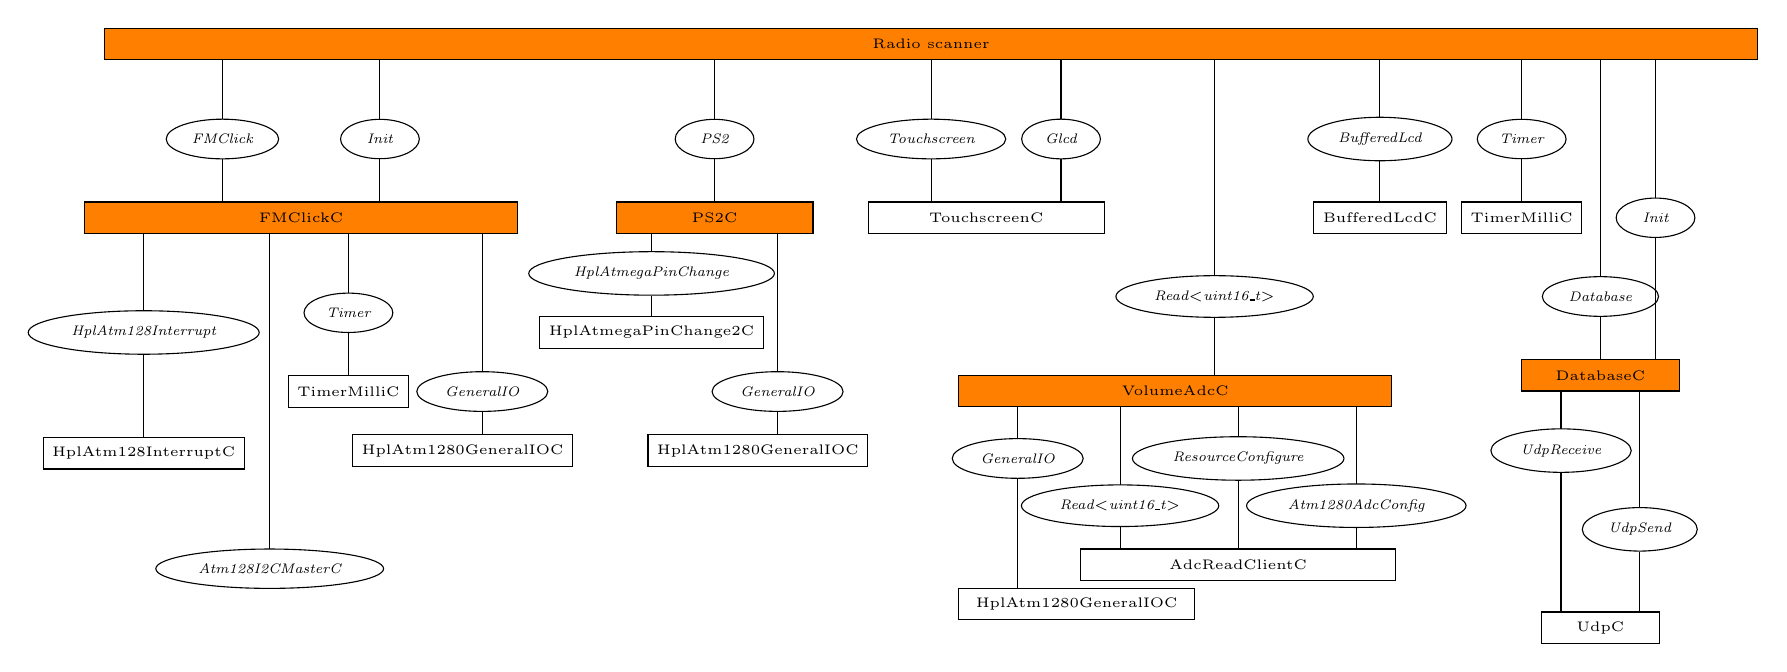
\begin{tikzpicture}[>=latex']
		\tikzstyle{basic}=[draw,fill=white]
		\tikzstyle{module}=[basic,rectangle, font={\tiny}, minimum width=1.5cm, minimum height=0.4cm]
		\tikzstyle{interface}=[basic,ellipse, font={\tiny\itshape},minimum width=1cm, minimum height=0.4cm, align=center]
		\tikzstyle{student}=[fill=orange]
		\coordinate (modGame) at (0,0);
		\node[module, student, anchor=south, minimum width=21.0cm] (labGame)
			at ($ (modGame) + (-2,0) $) {Radio scanner};

		% MP3
	%	\draw ($(modGame.south) + (-2.5,0)$) -- +(0,-1)
	%		node[interface] (intMp3) {MP3};

	%	\draw (intMp3) -- +(0,-1)
	%		node[module, student] (modVS1011e) {VS1011eC};

	%	\draw (modVS1011e) -- +(0,-1)
	%		node[interface] (intVS1011) {HplVS1011e};

	%	\draw (intVS1011) |- +(-0.5,-2.5) coordinate (cModHplVS1011);

	%	\node[module, minimum width=6cm] (modHplVS1011) at
	%		($ (cModHplVS1011) + (0,0) $) {HplVS1011eC};

		% MP3 -- Hpl

		% \draw ($(modHplVS1011.south) + (-2.5,0) $) -- +(0,-1.25)
		% 	node[interface] (intSpiByte) {SpiByte};

		% \draw ($(modHplVS1011.south) + (-1.5,0) $) -- +(0,-0.5)
		% 	node[interface] (intSpiPacket) {SpiPacket};

		% \draw ($(modHplVS1011.south) + (-0.5,0) $) -- +(0,-1.25)
		% 	node[interface] (intSpiControl) {SpiControl};

		% \draw ($(modHplVS1011.south) + ( 0.5,0) $) -- +(0,-0.5)
		% 	node[interface] (intSpiRessource) {Ressource};

		% \draw ($(modHplVS1011.south) + (2.25,0) $) -- +(0,-0.875)
		% 	node[interface] (intSpiIO) {GeneralIO};

		% \node[module, minimum width=3.5cm] (modSpi)
		% 	at ($(modHplVS1011.south) + (-1.0,-2) $) {Atm1280UsartSpiC};

		% \draw (intSpiIO) -- +(0,-1.125)
		% 	node[module] (modSpiIo) {HplAtm1280GeneralIOC};

		% \draw (intSpiPacket)    -- (intSpiPacket    |- modSpi.north);
		% \draw (intSpiByte)      -- (intSpiByte      |- modSpi.north);
		% \draw (intSpiControl)   -- (intSpiControl   |- modSpi.north);
		% \draw (intSpiRessource) -- (intSpiRessource |- modSpi.north);

		% Physics
%		\draw ($(modGame.south) + (-1.00,0)$) -- +(0,-2)
%			node[interface,student] (intPhysics) {Physics};
%
%		\draw (intPhysics) -- +(0,-2.25)
%			node[module,student] (modPhysics) {PhysicsC};
%
%		% Sdcard
%		\draw ($(modGame.south) + (-0.125,0)$) -- +(0,-2.75)
%			node[interface] (intSdcard) {Sdcard};
%
%		\draw (intSdcard) -- +(0,-0.75)
%			node[module] (modSdcard) {SdcardC};

		% GLCD
		\coordinate (touchbase) at ($ (modGame.south) + (-2.0,0) $);

		\draw ($(touchbase) + (1.65,0)$) -- +(0,-1)
			node[interface] (intGlcd) {Glcd};

		\draw (touchbase) -- +(0,-1)
			node[interface] (intTouch) {Touchscreen};

		\path ($(touchbase) + ( 0.70,0)$) -- +(0,-2)
			node[module, minimum width=3cm] (modTouch) {TouchscreenC};

		\draw (intGlcd)  -- (intGlcd  |- modTouch.north);
		\draw (intTouch) -- (intTouch |- modTouch.north);

		% BufferedLCD

		\draw ($(modGame.south) + (3.7,0)$) -- +(0,-1)
			node[interface] (intLcd) {BufferedLcd};

		\draw (intLcd) -- +(0,-1) node[module] (modLcd) {BufferedLcdC};

		% Timer
		\draw ($(modGame.south) + (5.5,0)$) -- +(0,-1)
			node[interface] (intTimer) {Timer};

		\draw (intTimer) -- +(0,-1)
			node[module] (modTimer) {TimerMilliC};

		% ADC
		\draw ($(modGame.south) + (1.6,0)$) -- +(0,-3)
			node[interface] (intVolRead) {Read$<$uint16\_t$>$};

		\draw (intVolRead) |- +(-0.5,-1.2)
			node[module, student, minimum width=5.5cm] (modVolume) {VolumeAdcC};

		\draw ($(modVolume.south) + ( 2.3,0) $) -- +(0,-1.25)
			node[interface] (intAdcCfg) {Atm1280AdcConfig};

		\draw ($(modVolume.south) + ( 0.8,0) $) -- +(0,-0.65)
			node[interface] (intResCfg) {ResourceConfigure};

		\draw ($(modVolume.south) + (-0.7,0) $) -- +(0,-1.25)
			node[interface] (intRead) {Read$<$uint16\_t$>$};

		\draw ($(modVolume.south) + (-2.00,0) $) -- +(0,-0.65)
			node[interface] (intAdcIO) {GeneralIO};

		\node[module, minimum width=3cm] (modAdcIO) at
			($(modVolume.south) + (-1.25,-2.5) $) {HplAtm1280GeneralIOC};

		\draw (intAdcIO) -- (intAdcIO |- modAdcIO.north);

		\node[module, minimum width=4cm] (modAdcIO) at
			($(modVolume.south) + (0.8,-2) $) {AdcReadClientC};

		\draw (intAdcCfg) -- (intAdcCfg |- modAdcIO.north);
		\draw (intResCfg) -- (intResCfg |- modAdcIO.north);
		\draw (intRead)   -- (intRead   |- modAdcIO.north);

		% PS2
		\draw ($(modGame.south) + (-4.75,0)$) -- +(0,-1)
			node[interface] (intPS2) {PS2};


		\draw (intPS2) -- +(0,-1)
			node[module, student, minimum width=2.5cm] (modPS2) {PS2C};

		\draw ($(modPS2.south) + ( 0.8,0) $) -- +(0,-2.00)
			node[interface] (intPS2IO) {GeneralIO};

		\draw ($(modPS2.south) + (-0.8,0) $) -- +(0,-0.5)
			node[interface] (intPS2Int) {HplAtmegaPinChange};

		\draw (intPS2IO) |- +(-0.25,-0.75)
			node[module] (modPS2IO) {HplAtm1280GeneralIOC};

		\draw (intPS2Int) -- +(0,-0.75)
			node[module] (modPS2Int) {HplAtmegaPinChange2C};

		% FMClick
		\draw ($(modGame.south) + (-11.0,0)$) -- +(0,-1)
			node[interface] (intLSM) {FMClick};

		\draw ($(modGame.south) + (-9.0,0)$) -- +(0,-1)
			node[interface] (intFMinit) {Init};

		\path ($(intLSM)+(1,0)$) -- +(0,-1)
			node[module, student, minimum width=5.5cm] (modLSM) {FMClickC};

		\draw (intLSM) -- +(0,-0.8);
		\draw (intFMinit) -- +(0,-0.8);
		\draw ($(modLSM.south)+(-0.4,0)$) -- +(-0.0,-4.25)
			node[interface] (intLSMI2C) {Atm128I2CMasterC};

		\draw ($(modLSM.south)+(-2.0,0)$) -- +(-0.0,-1.25)
			node[interface] (128int) {HplAtm128Interrupt};

		\draw ($(128int.south)+(-0.0,0)$) -- +(-0.0,-1.25)
			node[module] (128intC) {HplAtm128InterruptC};

		\draw ($(modLSM.south) + ( 2.3,0) $) -- +(0,-2.00)
			node[interface] (intPS2IO) {GeneralIO};

		\draw (intPS2IO) |- +(-0.25,-0.75)
			node[module] (modPS2IO) {HplAtm1280GeneralIOC};

		\draw ($(modLSM.south) + (0.6,0)$) -- +(0,-1)
			node[interface] (intTimer) {Timer};

		\draw (intTimer) -- +(0,-1)
			node[module] (modTimer) {TimerMilliC};
%		% random ADC
%
%		\draw ($(modRandom.south) + (-1,0)$) -- +(0,-0.60)
%			node[interface] (intRndRead) {Read$<$uint16\_t$>$};
%
%		\draw (intRndRead) |- +(-0.0,-1.2)
%			node[module, student, minimum width=5.5cm] (modRandAdc) {RandomAdcC};
%
%		\draw ($(modRandAdc.south) + ( 2.3,0) $) -- +(0,-1.25)
%			node[interface] (intRndAdcCfg) {Atm1280AdcConfig};
%
%		\draw ($(modRandAdc.south) + ( 0.8,0) $) -- +(0,-0.65)
%			node[interface] (intRndResCfg) {ResourceConfigure};
%
%		\draw ($(modRandAdc.south) + (-0.7,0) $) -- +(0,-1.25)
%			node[interface] (intRndRead) {Read$<$uint16\_t$>$};
%
%		\draw ($(modRandAdc.south) + (-2.00,0) $) -- +(0,-0.65)
%			node[interface] (intRndAdcIO) {GeneralIO};
%
%		\node[module, minimum width=3cm] (modRndAdcIO) at
%			($(modRandAdc.south) + (-1.25,-2.5) $) {HplAtm1280GeneralIOC};
%
%		\draw (intRndAdcIO) -- (intRndAdcIO |- modRndAdcIO.north);
%
%		\node[module, minimum width=4cm] (modRndAdcIO) at
%			($(modRandAdc.south) + (0.8,-2) $) {AdcReadClientC};
%
%		\draw (intRndAdcCfg) -- (intRndAdcCfg |- modRndAdcIO.north);
%		\draw (intRndResCfg) -- (intRndResCfg |- modRndAdcIO.north);
%		\draw (intRndRead)   -- (intRndRead   |- modRndAdcIO.north);

		% score

		\draw ($(modGame.south) + (6.5,0)$) -- +(0,-3)
			node[interface] (intchannellist) {Database};

		\draw ($(modGame.south) + (7.2,0)$) -- +(0,-2)
			node[interface] (intchannellistInit) {Init};


		\draw (intchannellist) -- +(0,-1)
			node[module, student, minimum width=2cm] (modchannellist)
			{DatabaseC};

		\draw ($(modchannellist.south) + (-0.5,0) $) -- +(0,-0.75)
			node[interface] (intUdpReceive) {UdpReceive};

		\draw ($(modchannellist.south) + ( 0.5,0) $) -- +(0,-1.75)
			node[interface] (intUdpSend) {UdpSend};

		\node[module] (modUdp) at ($(modchannellist.south) + (0,-3) $) {UdpC};

		\draw (intUdpSend)    -- (intUdpSend    |- modUdp.north);
		\draw (intUdpReceive) -- (intUdpReceive |- modUdp.north);
		\draw (intchannellistInit) -- (intchannellistInit |- modchannellist.north);

	\end{tikzpicture}lvatest-mcvl
}
\end{turn}
	\caption{Proposed interface architecture for the radio scanner}
	\label{fig:tinyos_software_stack}
\end{figure}
A proposal for the TinyOS modules used in the application is shown in
	\cref{fig:tinyos_software_stack}.
Square boxes mark configurations/modules while elliptic nodes denote
	interfaces.
The modules filled in orange have to be implemented by you, while the white
	modules are already provided by us respectively included in TinyOS.
Note that the interface proposal is not complete as, depending on your
	implementation, you might need additional modules and there might be other
	modules below the ones that are shown.
You can also change some module dependencies if they are useful.

\begin{note}
	The GLCD is wired by \module{TouchscreenC}.
\end{note}

The modules are explained in the following:

% -----------------------------------------------------------------------------
\subsection{Radio Application}
% -----------------------------------------------------------------------------

The application has implement at least the following functionality:
\begin{itemize}
	\item[(i)] On key press on the keyboard a search for the next radio station channel should start.
	\item[(ii)] A mode that lets you tune and then listen to a specific frequency.
	\item[(iii)] A key press that starts an automatic search through the whole bandwidth for all receivable radio channel
which is compiled into a list. 
	\item[(iv)] A key that adds the currently tuned radio channel to the, possibly empty, list.
If the channel is already in the list, the entry should be updated with the possible new information.
	%\item[(v)] A key that sets the current channel as default channel.
%You also have to assign a key to switch to the default channel.
	\item[(v)] A key that sets the current radio channel as favorite. Favorite
channels have to be accessed with keys 1-9 on the keyboard.
	\item[(vi)] It has to be possible to add a note to the channel via a inputs from the keypad.
	\item[(vii)] The GLCD has to display at least the following information about the current channel:
\begin{itemize}
\item frequency of the channel
\item RDS information if available (e.g., station name, radio text, time)
%\item some tag that shows if the channel is the default channel 
\item a number corresponding to the favorite list
\item the note
\end{itemize}
	\item[(viii)] The list has to be upated regularly (on demand or change of the channel list) on the workstation your board is connected to.
If the board is reset it has to sync with the workstation to
get a channel list.
%If the board gets a list from the workstation
%the default channel should be played.
	\item[(ix)] The current volume should be display on the LCD.
\end{itemize}

%% -----------------------------------------------------------------------------
\subsection{FMClickC (\interface{FMClick, Init})}
%% -----------------------------------------------------------------------------

This module interfaces with the FMClick add-on module
	via I2C.
It shall initialize the chip on boot and provide the radio information
	over the \interface{FMClick} interface.
The I2C communication with the chip is abstracted by the module
	\module{Atm128I2CMasterC}.
The FMClick module uses the \module{HplAtm1280GeneralIOC} to set up its input/output pins and
	\module{HplAtm128InterruptC} modules to handle external interrupts.
Detailed information on the specifics of the chip can be found in
	'Application 2 additional material'.
To get things started use the data sheet Si4702-03-C19 in combination with AN230 for initialization of the extension board.

Note that you must use 2 wire mode. Moreover, SEN pin is pulled to high by the board as we only have one fixed slave.
Furthermore, in our experience, having an internal buffer of the FMClick registers is a quite simple and efficient way to control the extension board. You simply load the register to your internal buffer then modify the buffer and write the buffer back to the module. 

\begin{lstlisting} [caption={Si4703},label=intf:Si4703]
typedef enum {
    PS, // Programm Station
    RT, // Radio Text
    TIME, // TIME
} RDSType;

interface FMClick {
    /**
     * tunes to a specific frequency
     */
    command error_t tune(uint16_t channel);

    /**
     * seek the next channel, either up or down
     */
    command error_t seek(bool up);

    /**
     * get the current frequency
     */
    command uint16_t getChannel(void);

    command error_t setVolume(uint8_t);

    /**
     * enable or disable RDS data
     */
    command error_t receiveRDS(bool enable);

    event void initDone(error_t res);

    /**
     * tuning is finished
     */
    async event void tuneComplete(uint16_t channel);

    /**
     * new RDS data is available
     */
    async event void rdsReceived(RDSType type, char *buf);
}
\end{lstlisting}

%To work with the chip, we recommend to first reset it by setting the bit
%	\textit{BOOT} in the register \textit{CTRL\_REG5\_A}.
%Following this, enable a sampling with \SI{50}{\hertz} of the x- and y-axis
%	via register \textit{CTRL\_REG1\_A}.
%After that, you can read the corresponding accelerometer values, e.g., for the
%	x-axis, from the registers \texttt{OUT\_X\_L\_A} and
%	\texttt{OUT\_X\_H\_A}.
%
%\begin{hint}
%	The chip has an auto-increment functionality.
%\end{hint}
%
%\begin{lstlisting} [caption={GamePad},label=intf:gamepad]
%interface GamePad {
%
%        command void request_linear_accel(void);
%
%        async event void linear_accel_ready(int16_t x_acc, int16_t y_acc);
%}
%\end{lstlisting}
%
%

% -----------------------------------------------------------------------------
\subsection{PS2C (\interface{PS2})}
% -----------------------------------------------------------------------------

The PS2 module uses the \module{HplAtm1280GeneralIOC} and
	\module{HplAtmPinChange2C} modules to set up its input pins and
	install an ISR for handling the clock generated by the keyboard's
	controller.

For every pressed key the keyboard generates so called scancodes.
These scancodes then need to be translated into a corresponding ASCII
	character.
As soon as the reception of one character is completed, the corresponding
	event should be fired to signal the received character to the main
	application.
You do not need to fire an event for every character (e.g., escape), but
	alphanumerical input, upper/lower case, and deletion must be supported.

Atmel Application Note 313~\cite{appnote:avr313} includes a scancode-to-ASCII
	mapping, and may provide you with some ideas on how to implement the
	interfacing of the PS/2 keyboard to the microcontroller.
Note that the code in the application note might not be the most efficient, or
	even easiest to implement for that matter.


\begin{lstlisting} [caption={PS2},label=intf:ps2]
interface PS2 {

	/**
	 * Init Pins, enable IRQ
	 */
	command void init(void);

	/**
	 * Fired when a character has been entered on the keyboard
	 *
	 * @param chr ASCII value of the character entered
	 */
	async event void receivedChar(uint8_t chr);

}
\end{lstlisting}

% -----------------------------------------------------------------------------
\subsection{VolumeAdcC ({\interface{Read}})}
% -----------------------------------------------------------------------------
\label{sec:voladc}

The module~\module{VolumeAdcC} provides the interface
	\interface{Read$<$uint16\_t$>$} and handles the access to the ADC for
	the volume adjustment of the MP3 playback.
The provided interface is a TinyOS standard interface and can be redirected
	directly to the module~\module{AdcReadClientC} which also handles the
	arbitration for the hardware access.
Additionally, the module~\module{AdcReadClientC} uses the
	interfaces~\interface{Atm1280AdcConfig} and \interface{ResouceConfigure},
	to trigger the pin setup after the ADC access is granted.
The pin access should be done by using the interface~\interface{GeneralIO}
	provided by the module~\module{HplAtm1280GeneralIOC} for all pins.

\begin{hint}
	All interfaces used by this module are defined by TinyOS.
	While hardware independent interfaces usually can be found in
	``tos/interfaces'' the hardware dependent interfaces (and their enum
	declarations) usually can be found under a path resembling
	``tos/chips[\_ecs]/\texttt{theChip}/[\texttt{theFunction}/]''.
	Note that code can be inherited from other chips.\\
	See ``support/make/platforms/bigAVR6\_1280.platform'' for details about
		the code locations for our platform.
\end{hint}



% -----------------------------------------------------------------------------
\subsection{TouchscreenC ({\interface{Glcd, TouchScreen}})}
% -----------------------------------------------------------------------------

The module \module{TouchscreenC} is provided by us and handles the output on
	the graphical LCD as well as the input via the resistive touchscreen.
For this reason, it provides two interfaces: \interface{Touchscreen} described
	in \cref{intf:touch} and \interface{Glcd} partly described in
	\cref{intf:glcd}.
The initialization of the module is directly wired to the \emph{SoftwareInit}
	stage of TinyOS.

The command \texttt{getCoordinates} requires a pointer to a place where the
	module can put the result.
Please note that the data is only valid after the event
	\texttt{coordinatesReady} was triggered.
For type definition of the variable type \emph{ts\_coordinates\_t} have a look
	at the corresponding header file.
There is also a demo in \texttt{apps\_ecs} that demonstrates the use of the
	touchscreen module.

\begin{note}
	The touchscreen needs to be calibrated.
	Please be aware that these two constants depend on the board.
	If you choose to add touchscreen UI, ensure that the ``sensitive'' areas
		are large enough to also work on another board.
\end{note}

\begin{lstlisting}[caption={TouchScreen},label=intf:touch]
interface TouchScreen{

    /**
     * Sets calibration offsets for the touchscreen
     * @return SUCCESS
     */
    command error_t calibrate( int8_t x_offset, int8_t y_offset );

    /**
     * Triggers request for touch coordinates
     * @param pointer to buffer for coordinates
     * @return SUCCESS if request was accepted
     *           EBUSY if another request is pending
     */
    command error_t getCoordinates( ts_coordinates_t *xy );

    /**
     * Notification that coordinates are ready
     */
    event void coordinatesReady( void );
}
\end{lstlisting}

\begin{lstlisting} [caption={GLCD},label=intf:glcd]
interface Glcd{

    /**
     * Set pixel
     * @param x-coordinate
     * @param y-coordinate
     * @return SUCCESS
     */
    command error_t setPixel(const uint8_t x, const uint8_t y);

    /**
     * Clear pixel
     * @param x-coordinate
     * @param y-coordinate
     * @return SUCCESS
     */
    command error_t clearPixel(const uint8_t x, const uint8_t y);

    /**
     * Invert pixel
     * @param x-coordinate
     * @param y-coordinate
     * @return SUCCESS
     */
    command error_t invertPixel(const uint8_t x, const uint8_t y);

    /**
     * Draw line
     * @param first point x
     * @param first point y
     * @param second point x
     * @param second point y
     * @return SUCCESS
     */
    command error_t drawLine(const uint8_t x1, const uint8_t y1,
                             const uint8_t x2, const uint8_t y2);

    /**
     * Draw rectangle
     * @param upper left x
     * @param upper left y
     * @param lower right x
     * @param lower right y
     * @return SUCCESS
     */
    command error_t drawRect(const uint8_t x1,const uint8_t y1,
                             const uint8_t x2,const uint8_t y2);

    ...

    /**
     * drawText
     * @param text
     * @param x-coordinate of lower left edge
     * @param y-coordinate of lower left edge
     * @return SUCCESS
     */
    command void drawText(const char *text,
                          const uint8_t x, const uint8_t y);

    /**
     * drawTextPgm
     * @param text stored in program memory
     * @param x-coordinate of lower left edge
     * @param y-coordinate of lower left edge
     * @return SUCCESS
     */
    command void drawTextPgm(const char *text,
                             const uint8_t x, const uint8_t y);
}
\end{lstlisting}

% -----------------------------------------------------------------------------
\subsection{TimerMilliC (\interface{Timer})}
% -----------------------------------------------------------------------------

Provides the \emph{Timer} interface you might need as system timer.
For a detailed description of the timer system in TinyOS please refer to the
		TinyOS documentation (especially the TinyOS programming manual and for
		more in-depth information TEP~102).

% -----------------------------------------------------------------------------
\subsection{BufferedLcdC (\interface{BufferedLcd})}
% -----------------------------------------------------------------------------

The module \module{BufferedLcdC} is given by us and handles the output on the
	2x16 character LCD.
It provides the interface \interface{BufferedLcd}.
The initialization of the module is directly wired to the \emph{SoftwareInit}
	stage of TinyOS.
There is also a demo in \texttt{apps\_ecs} that demonstrates the use of the
	2x16 LCD module.

\begin{lstlisting} [caption={BufferedLcd},label=intf:lcd]
interface BufferedLcd {

	/**
	 * @param period  refresh period in ms,
	 * 	set to 0 to disable auto refresh
	 */
	command void autoRefresh(uint32_t period);
	command void clear();
	command void write(char *string);
	command void write_P(prog_char *string);
	command void goTo(uint8_t line, uint8_t col);
	command void forceRefresh();

}
\end{lstlisting}

% -----------------------------------------------------------------------------
\subsection{UdpC ({\interface{UdpSend, UdpReceive}})}
% -----------------------------------------------------------------------------

This module is provided and implements the UDP communication.
The module is a generic component and takes a UDP port as parameter on
	initialization.
The module provides the interface \interface{UdpReceive}, using the UDP port
	from the initialization as listen port, as well as the interface
	\interface{UdpSend}, using the same UDP port as sender port.
It is possible to instantiate this component and only wire the receive
	interface and it is also possible to only wire the send interface.
Furthermore, it is possible to use multiple instances of the component in the
	same module (but with different port parameters).

There is a demo in the \texttt{apps\_ecs} folder demonstrating the use of the
	network stack.

To implement the whole functionality of the application you have to dig into
	the network stack so you can implement the ICMP echo reply as well as the
	proper rejection of UDP packets received on ports on which no module
	listens.
If you are changing something inside the network stack, please ensure that you
	copy the necessary file(s) into your application and make the changes
	there and not directly inside the provided module as stated in the general
	remarks at the beginning of this document.


\begin{note}
	For implementing the additional functionality you have to dig
		a little into the network stack and you have to know what to send
		when.
	However, the ratio between the points to get and the LOC to write is quite
		high.

	Important: When implementing the functions, recall the TinyOS programming
		hint about the forwarding of pointers!

	One last hint: the interface \interface{IpPacket} is wired by purpose.
\end{note}

For getting  an overview of  the network stack  you can use \emph{make
	bigAVR6\_1280 docs} or even\\ \emph{make bigAVR6\_1280 appdoc}.


% -----------------------------------------------------------------------------
\subsection{DatabaseC (\interface{Database, Init})}
% -----------------------------------------------------------------------------
This module is responsible for the communication with the workstation
	via UDP.
It provides interfaces \interface{Database} and \interface{Init}.
The following subsection the protocol for the UDP communication with the workstation is described. It starts with a list of available commands and a list of parameters for the commands.
The rest of the section explains how the commands should be used with a few examples.

%The used communication protocol is defined in \cref{tab:comproto}.
%It consists of a command to check basic connectivity (\texttt{ping}), a
%	command to acquire the current highscore (\texttt{get highscore}), and
%	commands to provide the scoreboard with information about the currently
%	active game.
%The protocol has the following format: \texttt{command parameter1
%	parameter2}.

%Note that the acquisition of the current database, will result in
%	multiple messages being sent by the server.
%Every entry is sent on its own, with the TODO information reihenfolge
%bestimmen.
%rank being at the start of the
%	message, followed by name and score which are divided by a '$-$'.
%The last entry in the database will be followed by \texttt{end channellist},
%	i.e., if there is currently no entry in the database a \texttt{end
%	channellist} will be send immediately.\\

\begin{lstlisting} [caption={Database},label=intf:Database]
typedef struct {
	// The quick dial key [1..9], pass 0 for no/deleting quick dial
    uint8_t quickDial,

    // The channels's frequency in multiplies of 100kHZ, for example, 99.9MHZ =
    // 999 * 100kHz => 999
    uint16_t frequency,

    // The RDS PI Program Idenfitifaction code
    uint16_t pi_code,

    // The channel name, length maximal 9 characters, normally the RDS PS field
    char *name,

    // optional notes of the channel (length maximal 40 characters) pass NUL
    // (\0) to delete exisiting notes or set none on new entries
    char *notes,
} channelInfo;


interface Database
{
	/**
	 * Save a new channel, or change properties of an existing one.
	 * @param id The channel index from the database store, 0xFF to autoselect,
     *           must be between 0 and 15 if passed manually
	 * @param channel The channel information, see channelInfo typedef
	 */
	command void saveChannel(uint8_t id, channelInfo *channel);


	/**
	 * Request the channel list from the database server
     * Received channels will be signaled through receivedChannelEntry
     * @param onlyFavorites tells server to send only the channels with a
     *        registered quickDial number, if not zero
	 */
	command void getChannelList(uint8_t onlyFavorites);

	/**
	 * Request the channel list from the database server
     * Received channels will be signaled through receivedChannelEntry
	 */
	command void getChannel(uint8_t id);

	/**
	 * Request that the Database purges all channels and their state
     * Received channels will be signaled through receivedChannelEntry
	 */
	command void purgeChannelList();

	/**
	 * Received an entry from the server.
	 * @param id The channel index from the database store
	 * @param channel The channel information, see channelInfo typedef
	 */
	event void receivedChannelEntry(uint8_t id, channelInfo channel);

	/**
	 * Server proceesed our request to save a Channel
     * @param id The channel index from the database store, the one we passed
     *           or the which was choosen if 0xFF was passed.
	 * @param result 0 = OK, 1 = No free index (only ID auto choose), 2 = DB error 
	 */
	event void savedChannel(uint8_t id, uint8_t result);
}
\end{lstlisting}



\subsubsection{Protocol}

\textbf{Command Overview}
\begin{description}
\item[add]       - adds a new entry, you'll get an ID as answer from the database
\item[update]    - updates an existing channel information entry in the database
\item[delete]    - delete a specific entry
\item[list]      - return a list of IDs which are saved in the database, optionally
             return only those with a quickDial setting
\item[get]       - returns all saved info from a specific ID
\item[purgeall]  - purges database with all it's info 
\end{description}
\textbf{Parameters}
\begin{description}
\item[id]     - unique id of entry (uint8\_t 0 $\leq$ id $\leq$ 15);
\item[name]   - name of the channel (fixed size 8 character ASCII sting)
\item[qdial]  - a quick dial/favorites number (uint8\_t 0 $<$ qdial $<$ 10)
\item[freq]   - channels frequency, uint16\_t as a multiple of 100 kHz
\item[picode] - the PI code from RDS (uint16\_t)
\item[note]   - a user chosen channel note (ASCII, dynamic length with max 40 characters) 
\end{description}
Each command consists of ASCII only characters ending with a single \textbackslash n (new line).
To separate command from parameters a single \textbackslash r (carriage return) is used between
command word and its parameters. Thus, any parameter value must ensure that neither
\textbackslash n or \textbackslash r is used by them.

Parameters consist of comma separated key=value pairs. To avoid the need to escape
characters used by the protocol itself (besides \textbackslash n) we expect a fixed size value
for the name parameter with a length of 8 characters and expect that the note
parameter is found at the end of the parameter list, as we switch off parsing and
just read until the command end control character \textbackslash n.
The order of the rest of the fields can be freely chosen.

Examples for commands:
\begin{itemize}
\item delete\textbackslash rid=2\textbackslash n
\item list\textbackslash r\textbackslash n
\end{itemize}
As answer you'll receive a message starting with either 'ok' or 'err', followed
by a carriage return (\textbackslash r) then an optional payload in the same format as described
above and a \textbackslash n to mark the end of the response.

If the answer is err there may be a single optional 'msg' paramter to explain the fault
($<$ 20 chars length ASCII).
For the add, update, delete and purgeall command an 'ok' result will have no parameter.
The get command follow the same parameter format and ordering as you'd use on a update
call, e.g., all fields available as key=value pairs.
The list command just returns a comma separated list of IDs, or no param if nothing
is available,

Examples for answers:
\begin{itemize}
\item for list:
  - ok\textbackslash r1,2,4,12\textbackslash n

\item for add:
\begin{itemize}
  \item  err\textbackslash rmsg=database full\textbackslash n\\
 \item ok\textbackslash r\textbackslash n
\end{itemize}
\item for get:
\begin{itemize}
  \item ok\textbackslash rid=1,name=Radio 78,freq=978,qdial=2,..\textbackslash n\\
  \item err\textbackslash rmsg=not exists\textbackslash n
\end{itemize}
\end{itemize}
Note that above's error message values are just examples. 

\section{Theory Tasks}

In the theory task we want you to develop argumentation skills that
     allow you to reason about the problem you have to solve and the
     solution you are designing.
Clear presentation of ideas is crucial for communication with team
     members, bosses, customers, etc.
This time we want you to prove your answers mathematically (by
     induction).
Points are solely awarded for proper mathematical argumentation.\\
\\
%%%%%%%%%%%%%%%%% new tasks %%%%%%%%%%%%%%%%%%%%%%%%%%%%%%%555
Setting:

A set of $n$ motes $\{p_1,\cdots,p_n\}$ is scattered in an area to broadcast data.
For simplicity, assume that every mote $p_i$ starts with a unique data sample $i$.
That is, mote $p_1$ starts with $1$, mote $p_2$ with $2$, and so on.

Communication is divided into several subsequent rounds and happens wirelessly via broadcasts.
Starting with round $r=1$, in each round every mote $i$ sends a broadcast message $m_i(r)$ to the system.
Broadcasting happens in zero time and all motes receive messages just before the next round starts.
A message $m_i(r)$ sent in round $r$ is the set of known data samples $S_i$. 
For example the message $m_1(1)$ sent by mote $1$ in round $1$ is $S_1=\{1\}$.
After receiving messages in some round $r$ mote $i$ updates the set of known data samples. 
E.g., if mote $p_i$ receives a message $m_j(r)$ from mote $p_j$ $S_i=S_i\cup S_j$.
This update is done for all received messages in each round.

This round-based communication can be modelled with a communication graph $G_r$
where each node in the graph represents a mote. 
A directed edge $(i,j)$ in $G_r$ represents that the message sent by mote $p_i$ in round $r$ was sucessfully received by mote $p_j$ in round $r$. 

\subsection*{Tasks} 

\begin{enumerate} 
	\item \pts{3 Points}{Strongly connected communication:}
		Assume that, because of message loss, not every message sent by a mote
		is received by every other mote. 
		The only guarantee the motes have is that in every round the
		communication graph is strongly connected.
		Show that after $n$ rounds of communication that data sample $1$ is part of every set $s_i$, i.e., $1 \in \bigcap_{i=1}^n S_i $.
\begin{figure}[h!]
\centering
	\begin{tikzpicture}
		\draw (0, 0.5) node (p1)    {$p_1$};
		\draw (-1, -1) node (p2)    {$p_2$};
		\draw (1, -1) node (p3)    {$p_3$};
		\draw[->] (p1) -- (p2);
		\draw[->] (p2) -- (p3);
		\draw[->] (p3) -- (p1);

		\draw (4, 0.5) node (p1)    {$p_1$};
		\draw (3, -1) node (p2)    {$p_2$};
		\draw (5, -1) node (p3)    {$p_3$};
		\draw[<->] (p1) -- (p2);
		\draw[<->] (p2) -- (p3);
		\draw[<->] (p3) -- (p1);

		\draw (8, 0.5) node (p1)    {$p_1$};
		\draw (7, -1) node (p2)    {$p_2$};
		\draw (9, -1) node (p3)    {$p_3$};
		\draw[<->] (p1) -- (p2);
		\draw[<->] (p2) -- (p3);	
	\end{tikzpicture}
	\caption{Example for $n=3$: three strongly connected graphs}
\end{figure}
	%\item \pts{1 Points}{Strongly connected communication extended:} 
	%	Under the same conditions as befor,
	%	how many rounds does it take for all motes to send the local unique data sample to all other motes \textbf(at most) (i.e. show that it is possible for $x$ rounds and not for $x-1$).
	\item \pts{2 Points}{Rooted tree communication:} Assume that,
		because of message loss, not every message send by a mote is received
		by every other mote. The only guarantee the motes have is that in every round
		the communication graph is a rooted tree, i.e., there exists at least one mote (the so called root mote) that has a directed path (a sequence of edges) to every other mote in $G_r$. Note that 		the root mote can be a different mote in every round.
		Show that after $n^2$ rounds of communication there exists a data sample $i$ that is part of every set $S_j$, i.e., $\{i\} \in \bigcap_{j=1}^n S_j $.
\begin{figure}[h!]
\centering
	\begin{tikzpicture}
		\draw (0, 0.5) node (p1)    {\textcolor{red}{$p_1$}};
		\draw (-1, -1) node (p2)    {$p_2$};
		\draw (1, -1)  node (p3)    {$p_3$};
		\draw[->] (p1) -- (p2);
		\draw[->] (p2) -- (p3);


		\draw (4, 0.5) node (p1)    {$p_1$};
		\draw (3, -1) node (p2)    {\textcolor{red}{$p_2$}};
		\draw (5, -1) node (p3)    {$p_3$};
		\draw[->] (p2) -- (p3);
		\draw[->] (p2) -- (p1);

	\end{tikzpicture}
	\caption{Example for $n=3$: two rooted trees}
\end{figure}
\end{enumerate}



\section{Demonstration and Protocol}

If you want points for your application, you have to submit a
	\texttt{*.tar.gz} archive to TUWEL until 20.01.2019, 23:59.
The name of the top-level folder of the archive must contain your
	matriculation number.
Inside the top-level folder place the Application folder from the template,
	and also include the Protocol folder with the Listing.pdf.
We enhanced the TinyOS build system with a target called \texttt{code} which
	generates  an appropriate archive.
Please consult the README as to where you have to change a few variables,
	e.g., set your name.

You are also obliged to participate in a delivery talk.
The delivery talks will be held between the 21.01.2019 and the 24.01.2019.
You must register in TUWEL for a \SI{30}{\minute} slot.
Please do so early, there are enough slots for everybody (and we will open
	additional ones if necessary) but we cannot accommodate everybody on the
	same day!

During the delivery talk, the tutor will download your application from TUWEL,
	check its functionality on the lab hardware, and will walk through your
	solution with you.
Be prepared that the tutor asks you questions about your implementation.
Only submissions that were approved by the tutor are considered by us.
We also require you to print out the first page of your Protocol (the adapted
version from the template is sufficient), sign it at the two indicated spots, and
give it to the tutor at the talk.

The lab Protocol itself should be written in \LaTeX{}, explaining your implementation
	and the decisions you made during implementation.
It should also contain a break-down of your working hours needed for the
	application and list which tasks required how much time (e.g.,
	reading manuals, implementation, debugging, writing the protocol, \dots).
A template for the layout of the code/protocol separation, including a \LaTeX{}
	template, is part of the git repository.
	%TODO
	%\url{http://ti.tuwien.ac.at/ecs/teaching/courses/mclu/misc/task1-specific-stuff/application-protocol-template-tar.gz/view}.
The protocol, including the solutions for the theory tasks if applicable, has
	to be submitted as a \texttt{*.tar.gz} archive to TUWEL until 27.01.2019,
	23:59.
The name of the top-level folder of the archive must be your
	matriculation number.
Inside the top-level folder place the Protocol folder from the template.
In addition to the \LaTeX{} files in the Protocol folder, include the
	Protocol.pdf in the Protocol folder!
The enhanced TinyOS Makefile provides a target \texttt{protocol} to generate
	an appropriate archive.

\subsection{Checklist}

\begin{itemize}
	\item Finish writing Application
	\item Check that the \texttt{listings.tex} in the Protocol folder includes
		all source files
	\item Generate a code archive via the provided Makefile target
		\texttt{code}
	\item Upload the archive to TUWEL
	\item Download the submission from TUWEL and
		\begin{enumerate}
			\item verify that the submission compiles in the lab and
			\item works on the target as intended.
		\end{enumerate}
	\item Finish writing the protocol and preparing for the make-up exam.
		Furthermore, participate in a delivery talk.
	\item Generate a lab protocol archive via the provided Makefile target
		\texttt{protocol}
	\item Upload the archive to TUWEL
	\item Download submission from TUWEL and check that all required files are
		included.
\end{itemize}

\section{Grading}\label{sec:grading}

Please note that the points below are upper bounds that are possible to reach.
However, there is always the possibility of point reduction due to exhaustive
	use of resources, not using sleep mode, not fulfilling specification,
	\dots

Therefore, if you aim for 20 points you should not gamble on dropping all
theory tasks.
Also remember the ``Collaboration Policy'' at the course web page which enacts
15 points deduction for cheating for everyone involved.
Discussion among students is encouraged, but this is no group task.
All programming and theory tasks have to be done on your own!

\vspace{10mm}

\begin{tabular}{|r|r p{8.5cm}|}
\hline
Points & Sub & Part\\
\hline
20 &   & Application \\
   & 4 & Radio scanner \\
   & 6 & FMClick  \\
   & 1 & ADC -- Volume \\
   & 3 & PS/2 \\
   & 4 & Database\\
   & 2 & clean TinyOS programming \\
\hline
\hline
5 &   & Theory Tasks (every task is evaluated separately).\\
\hline
\end{tabular}


\bibliographystyle{IEEEtran}
\bibliography{../../references}

\end{document}

